\label{sec:background}
\subsection{CNN-based methods for DSLAM}
As mentioned above, there are two essential components on each robot: $1)$ Visual Odometry (VO) and $2)$ Decentralized Place Recognition (DPR).


\begin{figure}[thb]  
    \centering  
    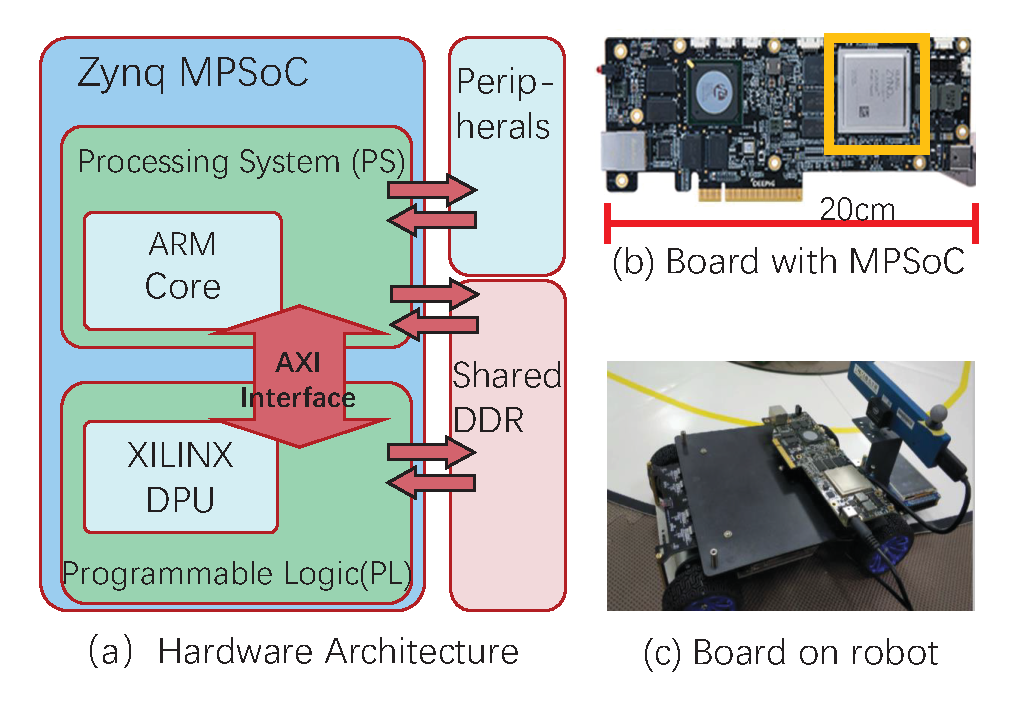
\includegraphics[width=0.95\linewidth]{fig/plps.eps}
    \caption{Xilinx Zynq Zu9 MPSoC Platform}
    \label{fig:plps}
\end{figure}

\subsubsection{Visual Odometry (VO)}

Visual odometry estimation is the task to infer ego-motion from a sequence of images and an essential component of the DSLAM system. Some feature-based SLAM systems have enjoyed great success, like ORB-SLAM \cite{DBLP:journals/trob/Mur-ArtalMT15} and ORB-SLAM2 \cite{Mur-Artal:2017281}. Recently, several studies have shown that these feature-based SLAM systems require high computing resources. Fang et al. \cite{Fang2017FPGAbasedOF} illustrate that the feature extraction stage is the most computation-intensive phase, consuming >50\% of CPU resources. In order to make full use of the parallelism of the embedded platform, a recent work \cite{Zhan:2018e92} introduces CNN for end-to-end pose 6-DoF estimation.

% As FPGA is one of the most promising platforms as the accelerator for VO, the SLAM system on FPGA has become a hot research topic. However, FPGA-accelerated feature extraction still consumes a lot of time and computing resources, which cannot be deployed simultaneously with an FPGA-accelerated neural network.

\subsubsection{Decentralized Place Recognition (DPR)}

The goal of place recognition or DPR is to calculate a given frame into a limited set of places. Every place can be encoded as compact code that can be easily transferred at low communication costs. Traditional location recognition methods typically convert input frames into a collection of hand-crafted feature points and local descriptors, such as SIFT \cite{Lowe:2004e6e} or ORB \cite{Mur-Artal:2017281}, using vectorization techniques like bag-of-words (BoW) \cite{Galvez-Lopez:2012c94}. 
Recent advances \cite{Arandjelovic:2017997, Noh:2017d0b} in the CNN enable powerful end-to-end model for place recognition, and NetVLAD is one of the best CNN-based methods to do DPR. 
% The NetVLAD algorithm based on VGG-16 \cite{Simonyan:20143be} model consumes more than $80G$ operations for a single $300 \times 300$ input image (each operation means addition or  multiplication). This makes NetVLAD very challenging to deploy on traditional embedded hardware platforms.

\subsection{Hardware architecture of Zync MPSoC}

The CNN-based VO and DPR components consume more than tens of billions of operations and thus are difficult to deploy on embedded systems. The Xilinx ZU9 MPSoC is a chip with ARM cores and FPGA fabric, and can be used to run CNN on embedded systems. The architecture of MPSoC is illustrated in \cref{fig:plps}.

The ARM cores with an embedded Linux operation system are called Processing System (PS). The FPGA fabric is called Programmable Logic (PL). The peripherals like camera and communication units (WiFi or others) are accessible to PS. The high-bandwidth on-chip AXI interface is used to communicate between PS and PL. PS and PL can also share DDR to transfer large amounts of data such as every frame of the camera.
Xilinx CNN accelerator, called DPU \cite{Tech:2019360}, is one of the state-of-the-art accelerators and is known for its energy efficiency in running various CNN structures. We deploy the DPU accelerator on the PL side of Zynq SoC.

Though FPGA can significantly improve the performance and energy efficiency of CNN inference, FPGA cannot efficiently calculate the floating-point number and requires fixed-point parameters and intermediate data in CNN.

% \subsection{Motivation}
% Though previous work \cite{Cieslewski:20187ee} proposes data-efficient DSLAM system, it is difficult to implement the two essential components, VO and place recognition simultaneously on a communication-limited and energy-constrained embedded hardware platform on a real robot. We propose this hardware-software co-design DSLAM system to use Xilinx Zynq MPSoC and Deephi DPU to execute these two components on the real system.

